% =====================================================================
%  Paper skeleton — Fleet Intelligence & HEMM Operations project
%  Compile:  pdflatex main && bibtex main && pdflatex main && pdflatex main
%            (or simply: latexmk -pdf main)
%  Class: IEEEtran (conference style, ships with MiKTeX/TeX Live).
% =====================================================================
\documentclass[conference]{IEEEtran}

% --- If IEEEtran.cls is unavailable, comment the line above and
%     uncomment the two lines below for a generic two-column layout ----
% \documentclass[10pt,twocolumn]{article}
% \usepackage[a4paper,margin=2cm]{geometry}

\usepackage[T1]{fontenc}
\usepackage[utf8]{inputenc}
\usepackage{graphicx}
\usepackage{amsmath,amssymb}
\usepackage{booktabs}
\usepackage{xcolor}
\usepackage{cite}
\usepackage[hidelinks]{hyperref}

\graphicspath{{figures/}}

% ---------- title & authors (EDIT AUTHORS) -----------------------------
\title{Fleet Intelligence for Autonomous HEMM Operations:\\
A Simulation-to-Learning Study of Truck Dispatch\\and ETA Prediction}

\author{
\IEEEauthorblockN{Author One\IEEEauthorrefmark{1}, Author Two\IEEEauthorrefmark{2}, Author Three\IEEEauthorrefmark{3}}
\IEEEauthorblockA{\IEEEauthorrefmark{1}Department / Institute, email@example.com}
\IEEEauthorblockA{\IEEEauthorrefmark{2}Department / Institute, email@example.com}
\IEEEauthorblockA{\IEEEauthorrefmark{3}Department / Institute, email@example.com}
}

\begin{document}
\maketitle

% =====================================================================
\begin{abstract}
Surface-mining productivity hinges on the dispatch of heavy earth-moving
machinery (HEMM) fleets: every truck assignment trades travel time against
loader queues and coal depletion. Learning-based dispatch and arrival-time
prediction are promising, but studying them requires an instrumented
environment that reproduces realistic fleet dynamics. We present an
end-to-end fleet-intelligence pipeline. First, a physics-based simulator in
which haul trucks---driven by iLQR model-predictive controllers with
cooperative collision avoidance and adaptive cruise following---operate
under a three-tier decision stack (global dispatch planner,
congestion-aware routing, local path tracking) on a $\sim$300-node mine
road network, logging per-second telemetry and lifecycle events. From 182
logged haulage cycles we build trip-level datasets and study ETA prediction
with models of increasing structure, from classical regressors to
GraphSAGE networks on the road graph. We then train four Double-DQN
dispatch architectures---central, per-truck, per-mine bidding, and a
universal mine--dump policy---under an identical fairness contract against
six hand-built policies, using the queue-aware rule ETA\_MIN as the primary
baseline and a perfect-foresight greedy rule as an oracle ceiling. All four
learned architectures beat ETA\_MIN by $+5.2\%$ to $+10.7\%$ mean reward,
and the best (per-mine bidding, $-267.4$) exceeds the oracle ceiling
($-272.3$). The results suggest that centralised value learning recovers
near-oracle dispatch quality from realistic observations alone.
\end{abstract}

\begin{IEEEkeywords}
Heavy earth-moving machinery (HEMM), fleet dispatch, autonomous haulage,
model predictive control, reinforcement learning, double DQN,
ETA prediction, graph neural networks, mining simulation.
\end{IEEEkeywords}

% =====================================================================
% ---------------------------------------------------------------------
\section{Introduction}
% GOAL OF THIS SECTION: motivate the work in 3-4 paragraphs + contributions.
% (1) Surface mining moves material with fleets of heavy earth-moving
%     machinery (HEMM); the quality of truck dispatch (which truck goes to
%     which loader/dump, when) directly drives productivity, fuel burn,
%     and queueing losses.
% (2) Industry trend toward autonomous haulage (AHS) makes dispatch a
%     *control/learning* problem rather than a human-radio problem.
% (3) Research gap: studying learning-based dispatch and ETA prediction
%     requires an instrumented environment that (a) reproduces realistic
%     fleet dynamics (routing, car-following, loader queues, K-turns at
%     dead-end spurs) and (b) produces ground-truth operational data.
% (4) What this paper does: we build such a simulator, log a trip-level
%     dataset, study ETA prediction with progressively richer models, and
%     run a controlled shootout of four RL dispatch architectures.
% ---------------------------------------------------------------------

% TODO: motivation paragraphs with citations, e.g. \cite{...}

Our contributions are:
\begin{itemize}
  \item A physics-based, instrumented HEMM fleet simulator with a
        three-tier decision stack (global dispatch planner, congestion-aware
        routing, iLQR model-predictive truck control) and scripted
        multi-point turn manoeuvres at dead-end loading spurs. % TODO: expand
  \item A reproducible data pipeline (per-second telemetry + lifecycle
        events $\rightarrow$ merged sessions $\rightarrow$ trip/KPI tables)
        yielding a ground-truth dataset of 182 haulage cycles. % TODO: update if regenerated
  \item An ETA-prediction study progressing from classical regressors to
        graph-feature models and GraphSAGE networks on the mine road graph. % TODO
  \item A controlled comparison of four Double-DQN dispatch architectures
        (central, per-truck, per-mine bidding, universal mine--dump) against
        six hand-built policies under an identical fairness contract, using
        ETA\_MIN as the primary beatable baseline and a perfect-foresight
        greedy policy as an oracle ceiling. % TODO
\end{itemize}

% TODO: one short paragraph describing the organisation of the paper.

% ---------------------------------------------------------------------
\section{Related Work}
% GOAL: position the paper. Suggested subsections below; 1 paragraph each.
% Add real citations in references.bib and cite them here.
% ---------------------------------------------------------------------

\subsection{Autonomous Haulage and Fleet Dispatch}
% TODO: industrial AHS systems, dispatch heuristics (nearest, queue-aware,
% ETA-based), operations research approaches (LP/MILP assignment, DP).

\subsection{Model Predictive Control for Heavy Vehicles}
% TODO: MPC / iLQR trajectory tracking, car-following / ACC logic,
% cooperative collision avoidance via shared planned trajectories.

\subsection{Travel-Time (ETA) Prediction}
% TODO: classical regressors, graph/road-network features, GNN-based
% ETA models (e.g. GraphSAGE \cite{hamilton2017graphsage}).

\subsection{Reinforcement Learning for Dispatch}
% TODO: value-based RL (DQN \cite{mnih2015human}, Double DQN
% \cite{vanhasselt2016deep}), centralised vs decentralised agent framings,
% semi-MDP formulations of dispatch decisions \cite{sutton2018reinforcement}.

% ---------------------------------------------------------------------
\section{Simulation Platform}
% GOAL: describe the environment everything else is built on.
% ---------------------------------------------------------------------

\subsection{Mine Layout and Road Network}
% TODO: describe the map: ~300 nodes / ~280 edges, 29 load zones, 26 dump
% zones, 2 fuel stations, regional pit clusters connected to a main hub;
% roads rendered and driven as Catmull-Rom splines stitched per route.
% TODO: add a figure: screenshot of the simulator / map viewer.
% \begin{figure}[t]
%   \centering
%   \includegraphics[width=\columnwidth]{map_overview.png}
%   \caption{Mine road network used in all experiments.}
%   \label{fig:map}
% \end{figure}

\subsection{Three-Tier Decision Stack}
% TODO: (1) global planner assigns per-truck target queues (DP-style
% lookahead optimiser or greedy); (2) dispatcher tracks coal, reservations,
% and builds a congestion-weighted road graph (1 Hz); (3) local planner
% (A*/BFS) routes on that graph; (4) each truck tracks its route with an
% iLQR MPC (20-step horizon, 10 Hz) using shared planned trajectories for
% cooperative collision avoidance, plus an ACC car-following layer with
% SAT-based collision prediction and scripted K-turns at spur terminals.

\subsection{Truck Physics and Operational States}
% TODO: bicycle kinematics, jerk/steer-rate limits, loaded/empty speed
% caps, GPS noise + Kalman filter, state machine
% (GOING\_TO\_ENDPOINT $\rightarrow$ LOADING $\rightarrow$ TURNING\_AROUND
% $\rightarrow$ RETURNING\_TO\_START $\rightarrow$ UNLOADING $\rightarrow$ ...).

\subsection{Key Parameters}
% TODO: verify/adjust values; source: Simulation/config.py
\begin{table}[t]
  \centering
  \caption{Main simulation parameters (edit to match final config).}
  \label{tab:sim-params}
  \begin{tabular}{ll}
    \toprule
    Parameter & Value \\
    \midrule
    Trucks (default fleet)      & 3 \\
    Empty / loaded speed cap    & 30 / 25 km/h \\
    Load / unload service time  & 3.0 s \\
    MPC horizon / rate          & 20 steps / 10 Hz \\
    Safety distance             & 8 m \\
    Physics step                & 1/60 s \\
    \bottomrule
  \end{tabular}
\end{table}

% ---------------------------------------------------------------------
\section{Data Collection and Analytics Pipeline}
% GOAL: explain how raw simulation becomes analysis-ready datasets.
% ---------------------------------------------------------------------

\subsection{Logging Layer}
% TODO: two CSV streams per session written by SimLogger:
%  * telemetry (1 Hz per truck): position, speed, acceleration, cargo,
%    operational state, current/target node, per-step fuel \& CO$_2$
%    (physics-derived proxy from traction power);
%  * events (edge-triggered): ARRIVE/LOAD/DEPART/UNLOAD lifecycle
%    transitions incl. per-trip fuel, CO$_2$ and duration in metadata.
% Mention: headless mode (--headless --speed 5) for fast collection.

\subsection{Session Merging and KPI Extraction}
% TODO: merge\_logs.py time-offsets sessions into one timeline with run
% tags; kpi\_extractor.py rebuilds per-trip records (6 lifecycle
% timestamps $\rightarrow$ 4 sub-durations) plus fleet KPIs (1-min bins),
% queue events, and idle periods.

\subsection{The Trip Dataset}
% TODO: 182 completed trips; mean duration 231.4 s (median 229.8,
% max 1689 --- long-tail congestion events); trips.csv schema table below
% (trim/adjust as needed).
\begin{table}[t]
  \centering
  \caption{Trip-level record schema (analysis/trips.csv).}
  \label{tab:trips-schema}
  \begin{tabular}{ll}
    \toprule
    Field group & Columns (examples) \\
    \midrule
    Identity     & trip\_id, run\_id, truck\_id, load\_zone, dump\_zone \\
    Timestamps   & depart\_time\_s \ldots unload\_complete\_s \\
    Durations    & travel\_to\_mine\_s, load\_wait\_s, travel\_to\_dump\_s, \\
                 & unload\_wait\_s, total\_trip\_duration\_s \\
    Payload      & cargo\_kg, fuel\_L, co2\_kg \\
    Graph feats. & road\_dist\_to\_mine\_m, detour\_factor (trips\_graph.csv) \\
    \bottomrule
  \end{tabular}
\end{table}

% TODO (optional): EDA findings --- route medians, queue behaviour,
% outlier trips; reference analysis/report_eda_task3.md.

% ---------------------------------------------------------------------
\section{ETA Prediction for Haulage Cycles}
% GOAL: the learning-to-predict-trip-duration study.
% ---------------------------------------------------------------------

\subsection{Problem Formulation and Features}
% TODO: target = total\_trip\_duration\_s; feature sets: categorical
% (zones, truck), operational (cargo, trip number), queue proxies
% (rolling queue depth), road-graph features (Dijkstra distances, detour
% factor), route-relative ratios.

\subsection{Classical Baselines}
% TODO: Linear Regression / Random Forest / Gradient Boosting with
% Leave-One-Out CV; best LOO-MAE $\approx$ 15.9 s ($\approx$ 7.4\% of the
% 213.7 s mean trip). Update with final numbers from
% analysis/eta\_model\_summary.txt.

\subsection{Graph Features and Queue-Aware Models (v2)}
% TODO: GroupKFold by run\_id to prevent session leakage; dispatch-time vs
% mid-trip prediction variants; reference analysis/eta\_v2\_summary.txt.

\subsection{Graph Neural Network Models}
% TODO: GraphSAGE over the road graph (node features: type, degree, edge
% weights; trip head on src/dst embeddings + trip features); LOO-CV vs
% holdout variants \cite{hamilton2017graphsage}.

% TODO: results table comparing model families (MAE / RMSE / \% of mean).

% ---------------------------------------------------------------------
\section{Learning to Dispatch: RL Architecture Shootout}
% GOAL: the central experiment --- which RL framing fits haul-truck dispatch?
% ---------------------------------------------------------------------

\subsection{A Fast Surrogate Environment}
% TODO: "calendar simulator" --- a trip reduced to 5 numbers (travel legs,
% queue waits, service) sampled from per-route medians fitted on the real
% 182 trips; event queue + FCFS loader booking + coal depletion;
% $\sim$1 ms/trip vs $\sim$77 s/trip in the full simulator.

\subsection{Candidate Architectures}
% TODO: Table of A/B/C/D (agents, action space, observation dims).
\begin{table}[t]
  \centering
  \caption{The four candidate dispatch architectures (Double DQN).}
  \label{tab:architectures}
  \begin{tabular}{llll}
    \toprule
    Method & Agents & Action space & Observation \\
    \midrule
    B one-for-all & 1 central  & mine (9)          & global fleet (49) \\
    A per-truck   & $N$ indep. & mine (9)          & per-truck (38)    \\
    C per-mine    & 9 bidders  & bid level (5)     & per-mine (7)      \\
    D universal   & 1 central  & mine$\times$dump (54, masked) & global+dump (55) \\
    \bottomrule
  \end{tabular}
\end{table}

\subsection{Fairness Contract}
% TODO: same env, reward $r=-\text{trip\_duration}/100$, 20-config eval
% suite (fleet 4--12 $\times$ coal scale 0.6--2.0), Double DQN
% $\gamma{=}0.97$, replay 50k, n-step 3, $\varepsilon$ 1.0$\to$0.05,
% target sync 500 \cite{vanhasselt2016deep,mnih2015human}.

\subsection{Baselines: Floor, Primary, and Oracle Ceiling}
% TODO: describe the six hand policies. Key framing:
%  * PRIMARY BASELINE = ETA_MIN (strongest beatable rule: queue-aware
%    cycle-time minimisation);
%  * ORACLE CEILING = GREEDY_NEAREST (reads the env's exact future queue
%    state --- no realistic dispatcher can match it);
%  * FLOOR = FIFO / LOAD_BALANCE / ROUND_ROBIN;
%  * note ETA_AWARE collapses onto ETA_MIN in this environment.
\begin{table}[t]
  \centering
  \caption{Hand-policy ladder (mean reward over the 20-config suite).}
  \label{tab:baseline-ladder}
  \begin{tabular}{llr}
    \toprule
    Role & Policy & Mean reward \\
    \midrule
    Oracle ceiling & GREEDY\_NEAREST & $-272.3$ \\
    \textbf{Primary baseline} & \textbf{ETA\_MIN} & $\mathbf{-299.5}$ \\
    Duplicate      & ETA\_AWARE      & $-299.5$ \\
    Floor          & LOAD\_BALANCE   & $-398.3$ \\
    Floor          & ROUND\_ROBIN    & $-399.6$ \\
    Floor          & FIFO            & $-404.5$ \\
    \bottomrule
  \end{tabular}
\end{table}

\begin{figure}[t]
  \centering
  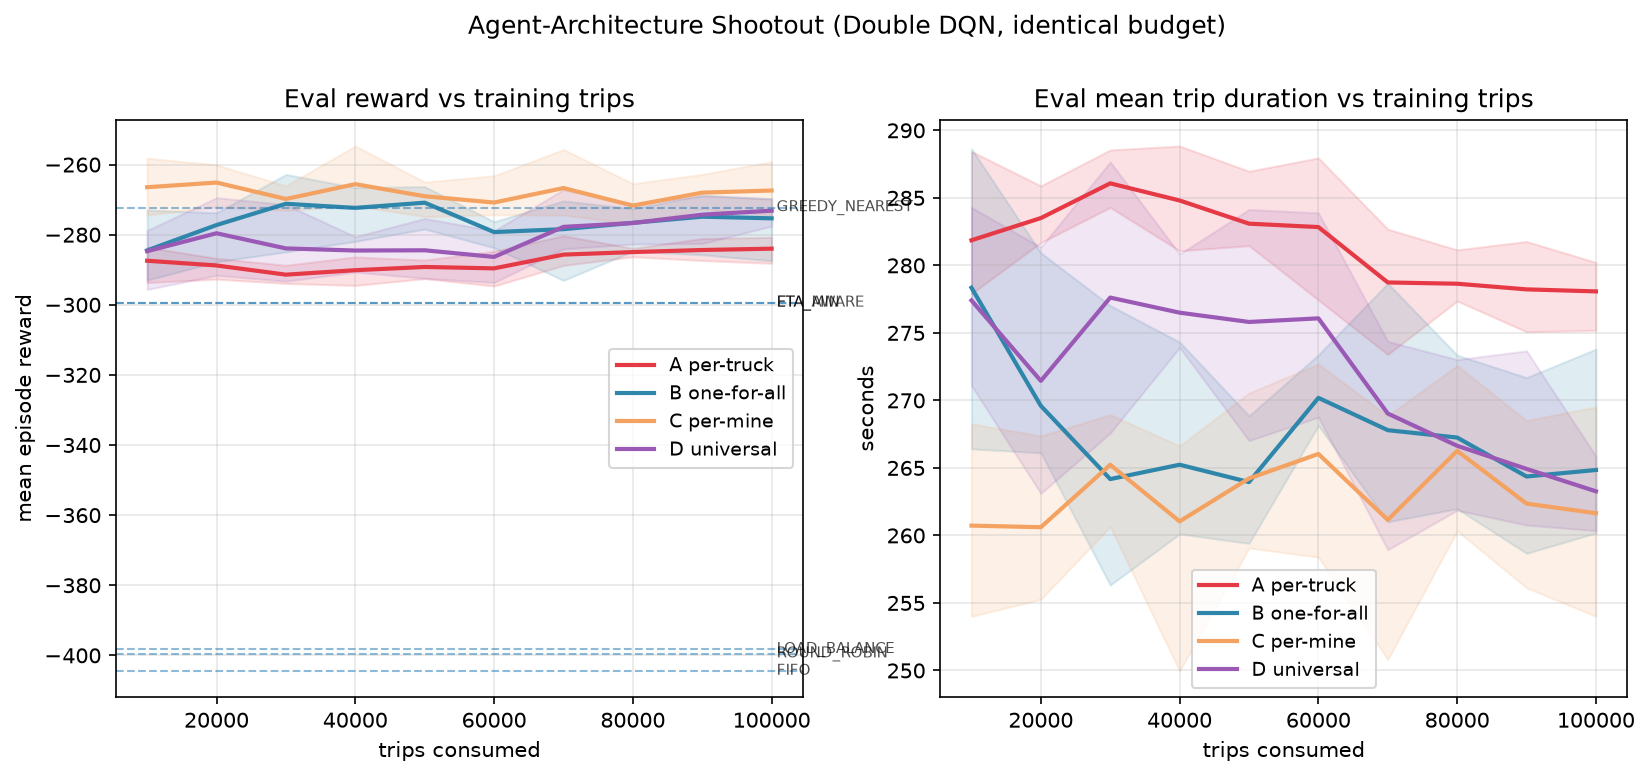
\includegraphics[width=\columnwidth]{learning_curves.png}
  \caption{Evaluation reward during training (mean over 5 seeds).
           Dashed lines: hand-policy references.}
  \label{fig:learning-curves}
\end{figure}

% ---------------------------------------------------------------------
\section{Results}
% GOAL: headline findings. Numbers below are the current 5-seed results;
% update if you retrain.
% ---------------------------------------------------------------------

% TODO: prose. Key facts to weave in (5-seed means, 100k training trips):
%  * ALL four RL architectures beat the primary baseline ETA_MIN on reward:
%      C per-mine  +10.7% (best mean: -267.4)
%      D universal  +8.8%
%      B one-for-all +8.1%
%      A per-truck  +5.2%
%  * Queue comparison is DISTANCE-NORMALISED (share of trip spent queuing =
%    wait/duration): C is the only method that also beats ETA_MIN here
%    (+13.5%); D (-19.1%), B (-20.8%), A (-51.9%) queue more per unit trip.
%    C therefore beats the baseline on ALL FOUR metrics.
%  * GREEDY oracle ceiling (-272.3): C's mean (-267.4) sits ABOVE it, i.e.
%    the learned policy exceeds myopic perfect-foresight dispatch.
%  * Seed stability: B has one collapsed seed (-287); C is most stable
%    (see Fig. \ref{fig:seed-spread}).
%  * Hypotheses H1-H4 (per README/report.py): summarise verdicts.

\begin{figure}[t]
  \centering
  
\includegraphics[width=\columnwidth]{6_vs_eta_min.png}
  \caption{RL architectures vs the primary baseline ETA\_MIN. Queue
           performance is distance-normalised (share of trip duration
           spent queuing), since queue exposure grows with trip length.}
  \label{fig:vs-baseline}
\end{figure}

\begin{figure}[t]
  \centering
  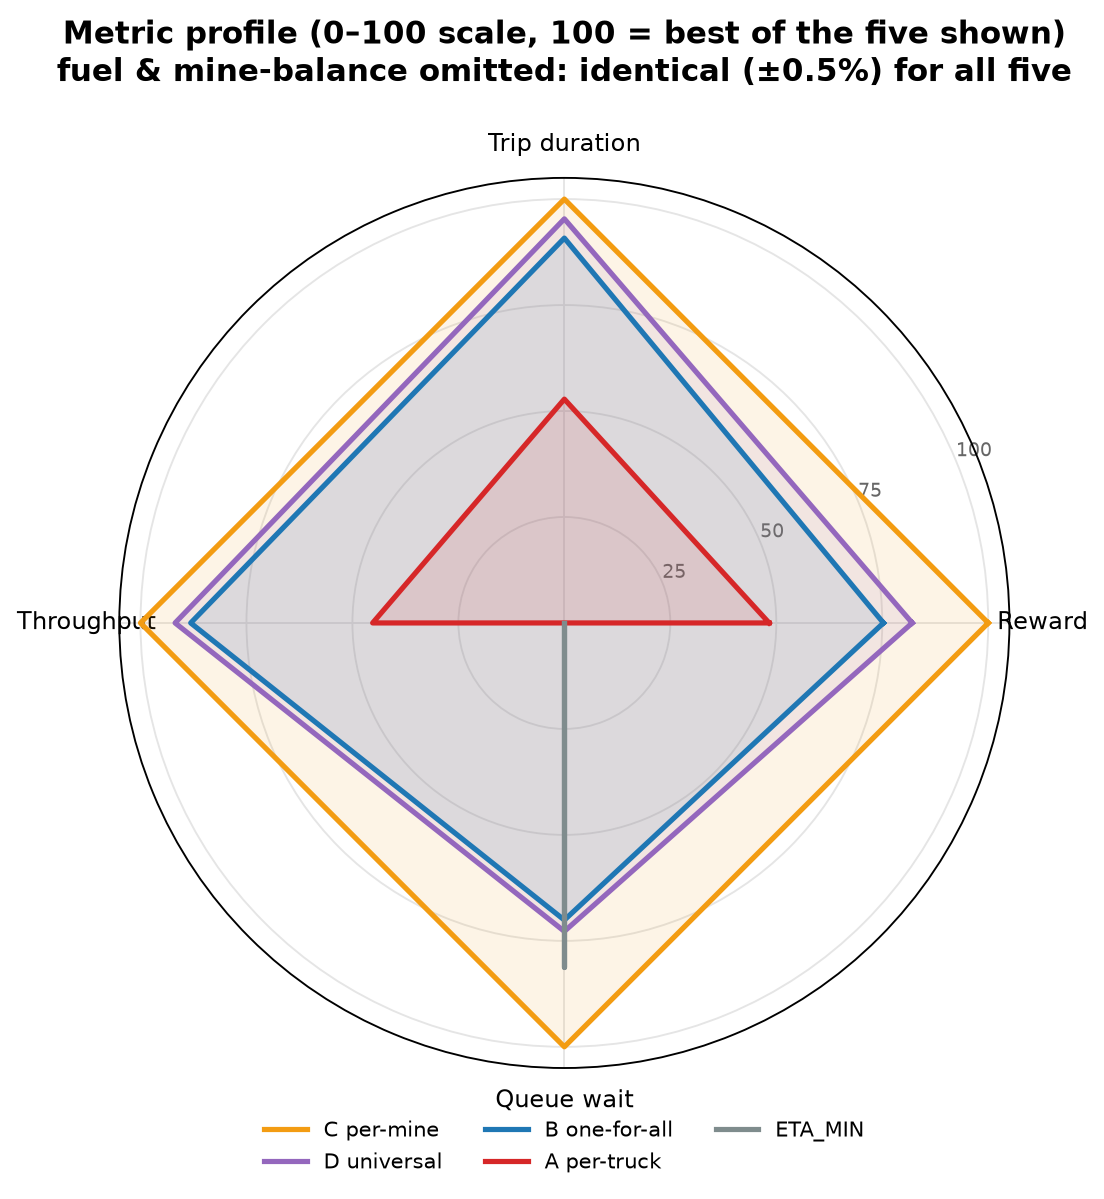
\includegraphics[width=\columnwidth]{2_radar_profile.png}
  \caption{Metric profiles of the four RL architectures against the
           primary baseline ETA\_MIN (0--100 scale per metric).}
  \label{fig:radar}
\end{figure}

\begin{figure}[t]
  \centering
  
\includegraphics[width=\columnwidth]{4_metric_heatmap.png}
  \caption{Scorecard across all methods and metrics (colour = 0--100 vs
           best/worst per column; number = actual value).}
  \label{fig:heatmap}
\end{figure}

\begin{figure}[t]
  \centering
  
\includegraphics[width=\columnwidth]{5_seed_spread.png}
  \caption{Seed-to-seed stability of final evaluation reward.
           ETA\_MIN = primary baseline; GREEDY = oracle ceiling.}
  \label{fig:seed-spread}
\end{figure}

\begin{figure}[t]
  \centering
  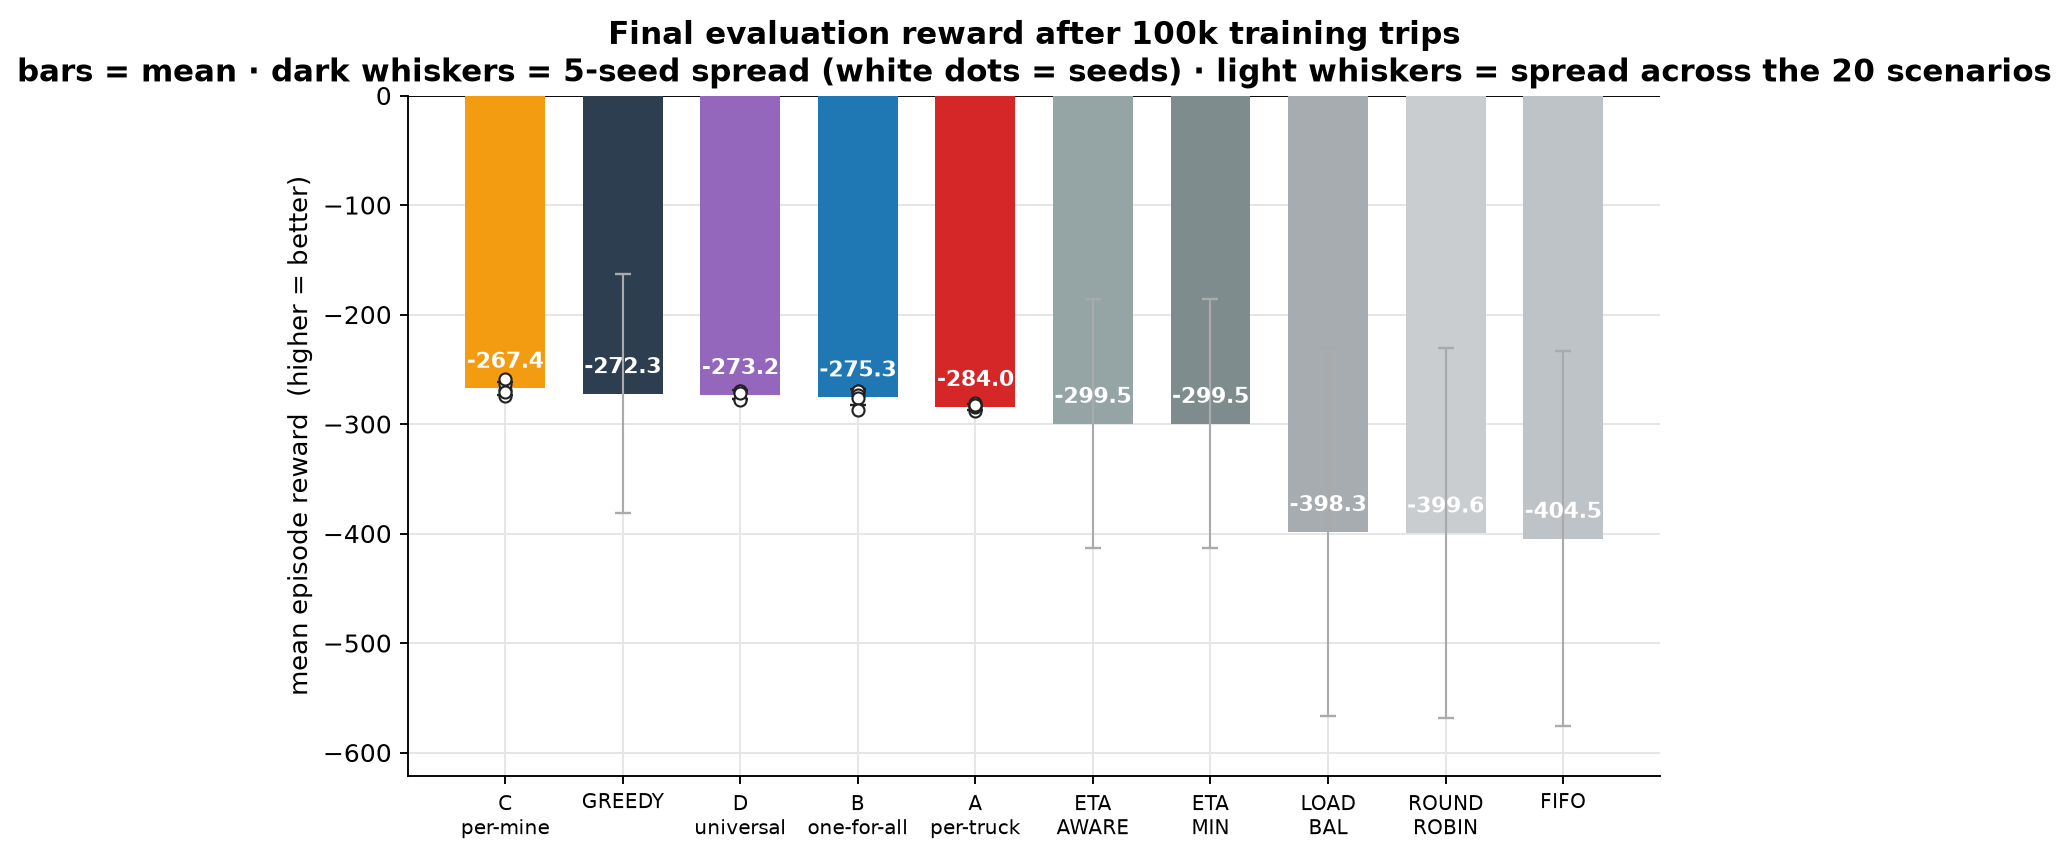
\includegraphics[width=\columnwidth]{1_reward_bar.png}
  \caption{Final evaluation reward of all methods after 100k training
           trips (bars = mean; dots = individual seeds).}
  \label{fig:reward-bar}
\end{figure}

% ---------------------------------------------------------------------
\section{Discussion}
% GOAL: honest interpretation + limitations.
% ---------------------------------------------------------------------

\subsection{Why Simple Heuristics Are Hard to Beat Here}
% TODO: reward = -duration; most of a trip's duration is fixed physics
% (distances, service times); the policy-controllable slice is thin, and
% queue-aware myopic rules (ETA_MIN) already capture most of it --- the
% total headroom from blind dispatch (FIFO -404.5) to the oracle (-272.3)
% is only ~130 reward points, and ETA_MIN captures ~80\% of it.
% Beating ETA_MIN by +5..11\% therefore means capturing nearly all
% remaining headroom, not a small gain.

\subsection{Limitations}
% TODO: (1) surrogate env fitted on real-trip medians with symmetric
% jitter -> rare emergent congestion (e.g. the 1689 s outlier trips) is
% under-represented; (2) ETA_AWARE degenerate in this env (residual
% bias $\approx$ 0); (3) full-fidelity sim currently validated at 3 trucks
% --- larger fleets stress the interaction layer (queues at single-lane
% spurs, K-turn conflicts); (4) fuel model is a physics proxy without
% grade/elevation.

\subsection{Threats to Validity}
% TODO: single map topology; median-calibrated timetable; eval on the
% same 20-config suite for all methods (fair but shared); seed variance.

\subsection{Future Work}
% TODO: multi-objective rewards (fuel, balance, queue externalities) that
% create genuine headroom over myopic rules; information-restricted
% baselines (naive vs oracle greedy); scaling the full-fidelity simulator
% to larger fleets; sim-to-real transfer discussion.

% ---------------------------------------------------------------------
\section{Conclusion}
% GOAL: 1 short paragraph + takeaway.
% ---------------------------------------------------------------------
% TODO: restate the pipeline (simulator -> data -> ETA models -> RL
% shootout), the headline result (all four RL architectures beat ETA_MIN,
% the strongest beatable hand rule, and approach the perfect-foresight
% oracle ceiling), and the design lesson (agent-framing matters less than
% the information structure of the problem; centralised value learning
% suffices to recover near-oracle dispatch on this task).


% =====================================================================
\bibliographystyle{IEEEtran}
\bibliography{references}

\end{document}
